\documentclass[crop,tikz]{standalone}

\usepackage{tikz}
\usetikzlibrary{decorations.pathmorphing,decorations.markings,calc}
\usetikzlibrary {angles,quotes}
\usepackage{makecell}
\usepackage{physics}

\begin{document}
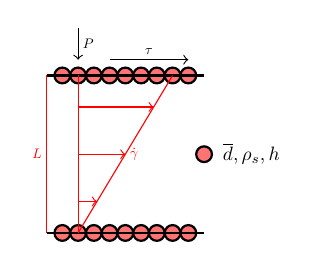
\begin{tikzpicture}[scale=2][font=\sffamily]
\foreach \x in { 0.1, 0.2,0.3, 0.4, 0.5,0.6, 0.7, 0.8, 0.9}
            \draw [color=black, fill=red!55, thick] (\x, 0) circle (0.05);

\foreach \x in { 0.1, 0.2,0.3, 0.4, 0.5,0.6, 0.7, 0.8, 0.9}
            \draw [color=black, fill=red!55, thick] (\x, 1) circle (0.05);


\draw [color=black, fill=red!55, thick] (1, 0.5) circle (0.05) node[scale = 0.7] at (1.3, 0.5){$\overline{d}, \rho_s, h$};

            
\draw[-, thick] (0, 1) -- (1, 1);

\draw[-, thick] (0, 0) -- (1, 0);



\draw[-, red] (0.2, 0) -- (0.2, 1);

\draw[-, red] (0.2, 0) -- (0.8, 1) node[midway, right, scale = 0.5] {$\Dot{\gamma}$};

\draw[->, red] (0.2, 0.2) -- (0.32, 0.2);
\draw[->, red] (0.2, 0.5) -- (0.5, 0.5);
\draw[->, red] (0.2, 0.8) -- (0.68, 0.8);

\draw[-, red] (0, 0) -- (0.0, 1) node[midway, left, scale = 0.5] {$L$}; 

\draw[->] (0.2, 1.3) -- (0.2, 1.1) node[midway, right, scale = 0.5] {$P$} ;

\draw[->] (0.4, 1.1) -- (0.9, 1.1) node[midway, above, scale = 0.5] {$\tau$};



\end{tikzpicture}
\end{document}